% !TeX root = ../main.tex
\section{Hand Evaluation, Monte Carlo, and Expert Systems}\label{sec:evaluation}

Before any strategic reasoning can occur, a program must answer two primitive questions quickly and exactly: \emph{which five-card hand does a player hold} (ranking), and \emph{how strong is a holding against a specified field of opponents} (equity). This section develops both primitives and then assembles them into the first rung of the algorithmic ladder: a rule-based expert system and a Monte Carlo simulation agent, the two paradigms that dominated computer poker before game-theoretic methods arrived.

\subsection{Exact hand evaluation}

A Hold'em evaluator is a function from seven cards to a totally ordered score. The natural construction exploits the fact that a player's effective hand is the \emph{best} of the $\binom{7}{5}=21$ five-card subsets:
\begin{equation}\label{eq:eval}
\operatorname{score}(c_1,\dots,c_7) \;=\; \max_{S \in \binom{[7]}{5}} \operatorname{rank}_5(S),
\end{equation}
where $\operatorname{rank}_5$ maps a five-card hand to a lexicographic tuple (category, primary kickers, \dots, final kicker). Because the nine categories of Section~\ref{sec:rankings} are mutually exclusive at fixed card multiplicity, and within-category comparison reduces to comparing kickers in order, $\operatorname{rank}_5$ takes values in a set of $7{,}462$ distinct equivalence classes, which pack into a single machine integer. Our implementation encodes $(\text{category}, k_1, k_2, \dots)$ as base-15 digits, so that \eqref{eq:eval} becomes 21 integer maximisations---about $1.5$\,ns per evaluation on commodity hardware. Production evaluators go further: the widely used two-plus-two table-driven evaluator precomputes multi-card lookup tables over the card space and evaluates seven cards in seven $O(1)$ table probes. The exact method matters little for correctness---all sound evaluators induce the same total order---but matters greatly for the training loops of Sections~\ref{sec:cfr} and~\ref{sec:rl}, whose wall-clock budgets are consumed almost entirely by evaluation.

\subsection{Monte Carlo equity estimation}\label{sec:mc}

Exact ranking solves showdowns, but decisions require \emph{equity}: the win probability of a holding against a distribution of opponent holdings and future boards. For a single uniformly random opponent this expectation has a closed form only in trivial cases; the standard tool is Monte Carlo estimation. Fix the player's hole cards $h$ and the visible board $B$, let $U$ denote the unseen cards, and let $e$ be the true equity. A \emph{runout} samples the opponent's hole cards $o \sim U$ and the board completion $r \sim U \setminus \{o\}$ uniformly without replacement; the estimator draws $n$ i.i.d.\ runouts and returns
\begin{equation}\label{eq:mcest}
\begin{split}
\hat e_n \;=\; \frac{1}{n}\sum_{i=1}^{n} W_i, \qquad
W_i \;=\;{}& \mathbf{1}\{\operatorname{score}(h \cup r_i) > \operatorname{score}(o_i \cup r_i)\} \\
&+ \tfrac{1}{m_i + 1}\,\mathbf{1}\{\text{tie against $m_i$ opponents}\},
\end{split}
\end{equation}
where $o_i$ is the sampled opponent holding, $r_i$ the sampled board completion, and a tie splits the pot among the $m_i + 1$ tied hands.

\begin{proposition}\label{prop:mc}
$\hat e_n$ is an unbiased estimator of $e$ with $\Var(\hat e_n) \le e(1-e)/n$, with equality when no ties occur. Consequently $\SE(\hat e_n) \le \sqrt{e(1-e)/n} \le \tfrac{1}{2\sqrt n}$, and by the de Moivre--Laplace central limit theorem an asymptotic $95\%$ confidence interval is $\hat e_n \pm 1.96\,\sqrt{\hat e_n(1-\hat e_n)/n}$.
\end{proposition}
\begin{proof}
Each $W_i$ is an independent draw of the random variable $W = \mathbf{1}\{\text{win}\} + \text{(fractional tie)}$, whose mean is $e$ by construction of the uniform sampling measure; ties contribute fractional mass so that $\E[W]$ equals the exact split-pot equity. Since $W \in [0,1]$ with $\E[W] = e$, the Bhatia--Davis bound gives $\Var(W) \le e(1-e)$, with equality exactly when $W$ is $\{0,1\}$-valued (no fractional ties); hence $\Var(\hat e_n) \le e(1-e)/n$, maximised at $e = 1/2$.
\end{proof}

The $1/\sqrt{n}$ decay is the governing constraint on every sampling-based poker agent: doubling precision quadruples the simulation budget. Figure~\ref{fig:mcprecision} plots the standard error \eqref{prop:mc} against $n$ and marks the two budgets used by our implementation: $n = 300$ for batch (tournament) play, giving $\SE \approx 2.9$ equity points, and $n = 1500$ for interactive play with a 220\,ms time budget, giving $\SE \approx 1.3$ points. The practical reading is sobering: even $1{,}500$ runouts cannot distinguish a $52\%$ equity from a $49\%$ equity at $95\%$ confidence, yet such margins decide most real bets. Variance-reduction techniques (antithetic pairing of high/low runouts, stratified sampling of opponent hands by canonical class) can shave constant factors, but the square-root wall is information-theoretic: an agent that wants sharper beliefs must either enumerate (exactly, at combinatorial cost) or \emph{condition on fewer unknowns}---which is precisely what the abstraction machinery of Section~\ref{sec:cfr} achieves by design.

\begin{figure}[htbp]
\centering
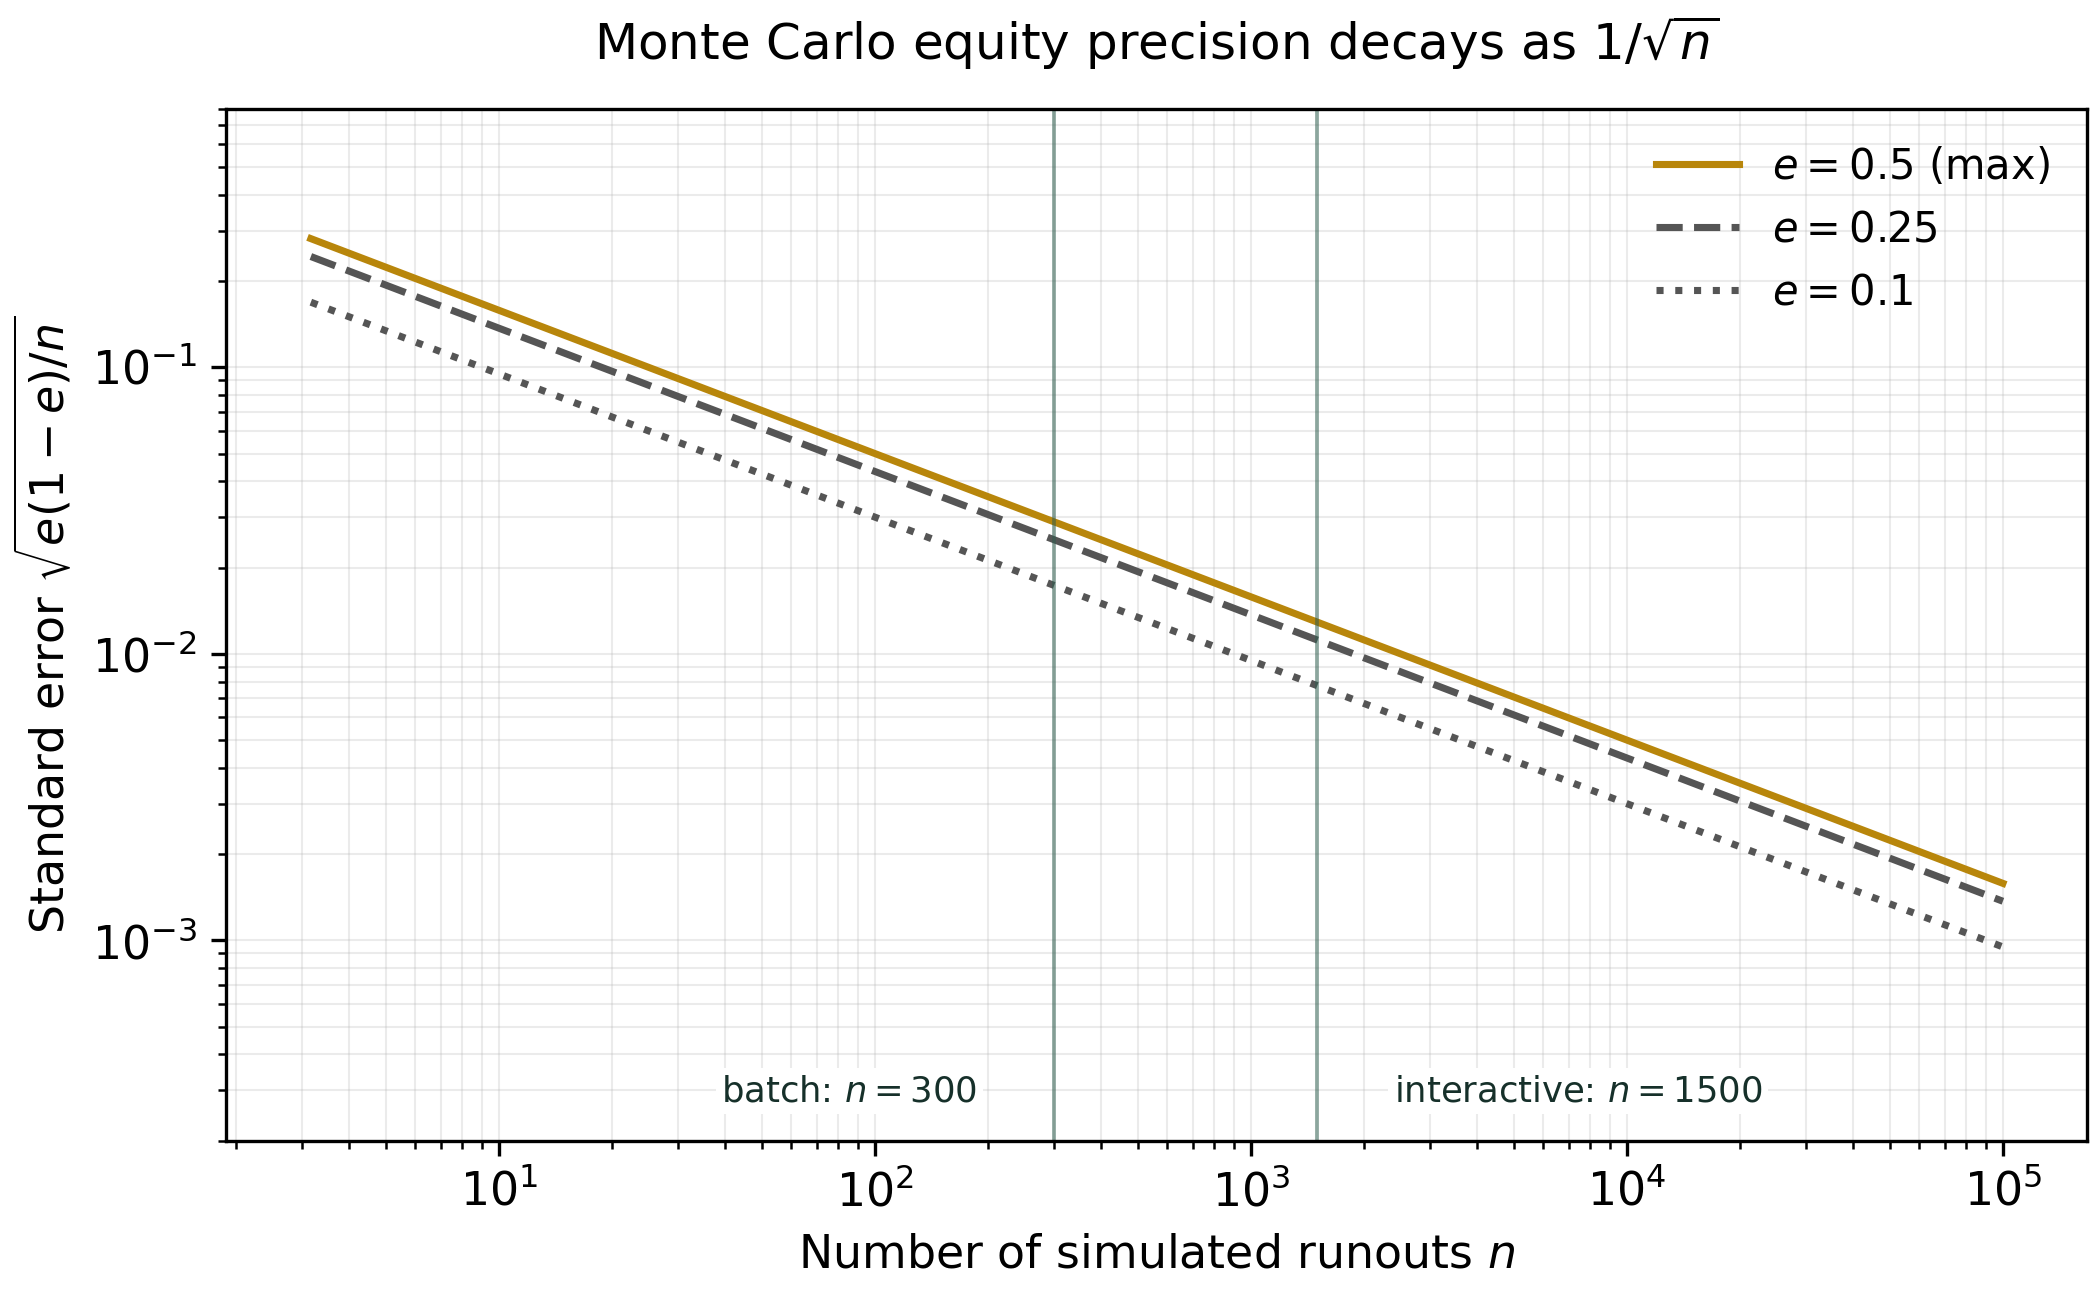
\includegraphics[width=0.82\textwidth]{figures/mc_precision.png}
\caption{Standard error of the Monte Carlo equity estimator \eqref{eq:mcest} as a function of the number of simulated runouts, for true equities $e \in \{0.5, 0.25, 0.1\}$ (the no-tie worst case). The vertical lines mark the two simulation budgets of our Monte Carlo agent: the batch budget $n = 300$ (worst-case $\SE \approx 2.9$ percentage points) and the interactive budget $n = 1500$ ($\SE \approx 1.3$ points).}
\label{fig:mcprecision}
\end{figure}

\subsection{Rule-based expert systems}

The oldest and still most common commercial paradigm encodes human expert knowledge as a decision procedure over computed statistics. Our implementation, which we call the \emph{rule agent}, is a faithful miniature of this school. At each decision point it computes three quantities: a \emph{strength} estimate $s \in [0,1)$---preflop, a table lookup of the 169 canonical hands' Monte Carlo equities (Figure~\ref{fig:preflop}); postflop, a made-hand percentile with additive draw bonuses---a \emph{position class} from $\{\text{EP}, \text{MP}, \text{LP}, \text{SB}, \text{BB}\}$, and the \emph{pot-odds threshold} $b/(P+b)$ of \eqref{eq:potodds}. Decision rules then combine them: open-raise when $s$ clears a position-dependent threshold (tighter in early position, looser on the button), three-bet premium holdings, call when $s$ exceeds the required equity plus a multiway safety margin $0.03 + 0.025\,\min(3, \text{opponents})$, value-bet strong made hands, and bluff at a low fixed frequency when last to act. Algorithm~\ref{alg:rule} gives the complete decision procedure.

\begin{algorithm}[htbp]
\DontPrintSemicolon
\caption{Rule-based decision at one betting node (our \emph{rule agent}; rules are priority-ordered, first match fires).}\label{alg:rule}
\KwIn{state (hole, board, pot $P$, to-call $b$, position $\rho$, opponents $m$), random draw $r \sim U(0,1)$}
\KwOut{action $\in$ \{fold, check/call, raise $\tfrac12$-pot, raise pot\}}
$s \leftarrow$ preflop-equity lookup or made-hand percentile $+$ draw bonuses\;
\If{$b = 0$}{
  \uIf{preflop \textbf{and} $s \ge \theta_{\text{open}}(\rho)$}{
    \eIf{$s \ge 0.62$ \textbf{and} $r < 0.35$}{emit pot-sized raise}{emit half-pot raise}\;
  }
  \uElseIf{postflop \textbf{and} $s \ge 0.84$}{
    \eIf{$r < 0.4$}{emit pot-sized raise}{emit half-pot raise}\;
  }
  \uElseIf{postflop \textbf{and} $s \ge 0.72$}{emit half-pot raise (value bet)\;}
  \uElseIf{postflop \textbf{and} $s \ge 0.56$ \textbf{and} $r < 0.45$}{emit half-pot raise (probe)\;}
  \uElseIf{postflop \textbf{and} $\rho = \mathrm{LP}$ \textbf{and} $s < 0.45$ \textbf{and} $r < 0.16$}{emit half-pot raise (bluff)\;}
  \Else{check (fold-option hands check behind)\;}
}
\Else{
  $\theta \leftarrow b/(P+b) + 0.03 + 0.025\min(3,m) - \mathbb{1}[\rho \in \{\text{SB},\text{BB}\}]\cdot 0.02$\;
  \If{preflop \textbf{and} $s \ge 0.68$ \textbf{and} raises this street $< 3$ \textbf{and} $r < 0.55$}{emit 3-bet\;}
  \If{postflop \textbf{and} $s \ge 0.80$ \textbf{and} raises this street $< 2$ \textbf{and} $r < 0.4$}{emit raise\;}
  \If{$s \ge \theta$}{call\;}
  \If{$b/(P+b) < 0.15$ \textbf{and} $s \ge 0.42$}{call (cheap peeling / set-mining)\;}
  \If{$b/(P+b) < 0.22$ \textbf{and} $s \ge b/(P+b) - 0.04$ \textbf{and} $r < 0.5$}{call (implied odds)\;}
  \Return fold\;
}
\end{algorithm}

The strengths of this paradigm are transparency (every action is explainable in terms a human recognises---the agent's user interface displays exactly these threshold comparisons), speed (microseconds per decision), and robustness against catastrophic error. Its weaknesses are equally structural. First, the thresholds are \emph{static}: the agent cannot adapt to an opponent who folds too much or calls too much, whereas a best responder profits precisely from such regularities. Second, and more fundamentally, the rule agent has no theory of \emph{balanced ranges}: because its aggression depends only on its own card strength, its betting ranges are transparently polarised or merged, and its bluff frequency is an arbitrary constant rather than a quantity chosen to make the opponent indifferent. A game-theoretic opponent can therefore exploit it systematically, a defect that Section~\ref{sec:experiments} quantifies in win-rate terms. The Monte Carlo agent improves the \emph{estimation} half of the problem---it replaces the heuristic strength $s$ with a live simulation against the actual number of opponents, with an honest confidence interval---but inherits the same static decision thresholds, so its fate against adaptive opponents is similar.

Both paradigms share a deeper limitation: they treat each decision in isolation, as a myopic expected-value calculation against a \emph{fixed} model of the opponents. Poker's central difficulty is that the model is not fixed---opponents' strategies respond to ours, and their private cards generate adversarial uncertainty that no amount of sampling removes. Formalising this observation requires the language of game theory, to which we now turn.
